Este capítulo apresenta os principais conceitos relacionados com a tecnologia blockchain e a forma como cada um deles contribui para a manutenção de suas propriedades. Apesar de existirem diversas variações entre as blockchains, este capítulo tem como foco as plataformas Bitcoin e Ethereum, a primeira por ter sido a pioneira da tecnologia blockchain e a mais conhecida até os dias atuais, e a última por estar diretamente relacionada com este trabalho. Além de expor os aspectos estruturais e funcionais da Ethereum, este capítulo também descreve sobre contratos inteligentes e vulnerabilidades existentes, fornecendo um conjunto de conceitos e informações necessárias para o entendimento da proposta deste trabalho.

Na Seção~\ref{tex:fund:blockchain} são introduzidos os fundamentos da tecnologia blockchain. Na Seção~\ref{tex:fund:ethereum} são abordados os conceitos e as particularidades inerentes à blockchain Ethereum. Na Seção~\ref{tex:fund:ethereum:smartc} é discutido sobre o ciclo de execução dos contratos inteligentes, vulnerabilidades presentes em contratos inteligentes, e ataques ocorridos que exploraram essas vulnerabilidades.

%---------------------------------------------------------------------%
\section{Sistemas distribuídos e a tecnologia Blockchain} \label{tex:fund:blockchain}

Ao implementar um sistema de \textit{software}, uma decisão fundamental a ser tomada diz respeito à sua arquitetura, isto é, o modo como seus componentes são organizados e se relacionam. As principais abordagens são as arquiteturas distribuída e centralizada~\cite{tanembaum2007sistemas}.

Em uma arquitetura centralizada, os componentes do sistema são dispostos em torno de um componente central e estão conectados a eles. Esses componentes centrais podem ser servidores, bancos de dados, centrais de controle, centrais de processamento ou qualquer elemento que concentre serviços ou recursos computacionais. Em contraste, em sistemas distribuídos não há nenhum elemento central para coordenação ou controle, de modo que seus elementos formam uma rede de componentes conectados que, de alguma forma, trabalham para manter o funcionamento do sistema~\cite{tanembaum2007sistemas}.

Quando os componentes de um sistema estão distribuídos entre vários computadores conectados, os recursos desses computadores são agregados ao sistema como um todo e disponibilizados diretamente a outros nós. Assim, os participantes do sistema atuam tanto como fornecedores quanto consumidores de recursos. Esse tipo de sistema distribuído é conhecido como sistema ponto a ponto~\cite{tanembaum2007sistemas}.

Em sistemas centralizados, recursos como processamento e armazenamento são delegados a apenas um computador central ou um conjunto específico de computadores. Podem haver também abordagens híbridas, nas quais os recursos computacionais são usados de forma distribuídas, mas alguns serviços, como gerenciamento de comunicação, geração de relatórios e tarefas de coordenação, por exemplo, são desempenhados por algum componente específico. Quando um sistema ponto a ponto não possui nenhum elemento central para controle ou coordenação, então este é considerado também como um sistema ponto a ponto puramente distribuído~\cite{tanembaum2007sistemas}.

Em sistemas distribuídos, a integração de recursos e serviços entre os componentes envolvidos, também chamados de nós do sistema, agrega diversos benefícios. Nesses sistemas, a capacidade total de processamento resulta da combinação da capacidade de processamento de todos os nós conectados. Assim, o poder computacional do sistema pode expandir-se se acordo com a demanda, bastando apenas conectar mais computadores ao sistema, o que agrega ao sistema a capacidade de expandir-se naturalmente. Desta forma, é comum que sistemas distribuídos tenham um poder de processamento maior do que um supercomputador individual. Com vários nós integrando o sistema, simplifica-se também a manutenção, pois substituir ou desativar computadores individuais de um sistema distribuído pode ser feito sem um impacto significativo no sistema como um todo. Este último fator eleva a confiabilidade no funcionamento do sistema, que pode continuar operando normalmente mesmo que máquinas individuais falhem~\cite{tanembaum2007sistemas, overview-blockchainbasic2018drescher}.

Apesar dos benefícios, em uma arquitetura distribuída é necessário lidar com uma série de questões. Sem entidades centrais para coordenar seus membros, a coordenação em um sistema distribuído deve ser feita pelos próprios nós participantes do sistema. Para que essa coordenação possa ser desempenhada é necessário um protocolo de comunicação, e lidar com os custos de processamento envolvidos no envio, recepção e processamento de mensagens. Essa necessidade constante de comunicação resulta em uma dependência das redes, que têm seus próprios desafios e adversidades. Como a comunicação em rede implica no envio e compartilhamento de dados críticos, entidades não confiáveis podem utilizar indevidamente a rede a fim de acessar e explorar informações, o que compromete a integridade do sistema~\cite{tanembaum2007sistemas, overview-blockchainbasic2018drescher}.

Resolver um problema de computação e prover serviços para usuários de computadores envolve a escrita de programas e \textit{softwares}. Quando se trata de sistemas distribuídos, esse processo implica em lidar com problemas de coordenação, comunicação, utilização de redes e segurança~\cite{overview-blockchainbasic2018drescher}. A forma como se lida com esses problemas impacta diretamente na integridade de um sistema.

%Sistemas de \textit{software} podem exercer diversas funções. Cada função pode ser implementada de diversas forma, no que diz respeito à segurança, comportamento esperado, facilidade de uso, entre outros aspectos. A maneira como são definidas as funções que um sistema de \textit{software} deve exercer e a forma como cada uma dessas funções deve funcionar depende da definição dos aspectos funcionais e não funcionais. Os aspectos funcionais especificam quais funções técnicas o sistema o sistema deve exercer, por exemplo, ler o código de barras de um boleto, tirar uma foto, processar pixeis de uma imagem e enviar e-mails. Os aspectos não funcionais definem como essas funções devem ser implementadas, por exemplo, ter uma interface gráfica intuitiva, ter boa performance, manter a integridade e a segurança.

A integridade é um aspecto esperado em qualquer sistema de \textit{software}, e engloba três componentes: integridade de dados; integridade comportamental; e segurança. A integridade de dados assegura que os dados usados e mantidos pelo sistema são completos, corretos e livres de contradições. A integridade comportamental garante que o sistema executa suas funções e rotinas de acordo com o esperado, sem falhas ou erros de lógica. A segurança atesta que o acesso às funcionalidades, dados dos usuários e dados internos do sistema estão restritos somente aos usuários autorizados~\cite{tanembaum2007sistemas}. 

A relação entre sistemas ponto a ponto puramente distribuídos e a tecnologia blockchain está em seu uso para prover e manter a integridade desses sistemas~\cite{overview-blockchainbasic2018drescher}. No trabalho pioneiro de \citeonline{overview-bitcoin2008nakamoto}, foi proposto uma solução para manter a integridade em uma versão ponto a ponto e puramente distribuída de um dinheiro eletrônico (ou criptomoeda) para pagamentos \textit{online} diretamente entre as duas partes envolvidas na transação, sem a necessidade de uma terceira parte intermediadora, como uma instituição financeira. A solução foi proposta com o objetivo de evitar o problema do gasto duplo, quando uma das partes envolvidas na transação executa a mesma transferência duas vezes para obter benefícios indevidos.

Para que os participantes desse sistema de pagamentos confiem na integridade do sistema, é preciso acessar o histórico das transações realizadas. Desta forma, o próprio participante, chamado também de nó participante, pode conferir a integridade das transações. Contudo, é necessário também que todos os nós tenham acesso ao mesmo histórico de transações.

Em empresas, utiliza-se um livro-razão para lançamento de registros contábeis para elaboração de relatórios financeiros~\cite{marion1985contabilidade}. Na estrutura de dados de uma blockchain, este livro-razão fica disposto por meio uma cadeia de blocos interligados (i.e., uma lista encadeada) que armazenam todo o histórico de transações. Cada nó da rede é responsável por manter uma versão atualizada do histórico de transações, assim como preservar a integridade dessas informações.

Para garantir a disponibilidade do mesmo histórico de transações para todos os nós. Sempre que uma nova transação ocorre, as informações sobre essa transação, como as contas envolvidas, a quantia transferida e o horário da transação, são transmitidas entre todos os nós da rede. Os nós participantes da rede, conhecidos também como mineradores, coletam uma determinada quantidade de transações e as englobam em um componente chamado de bloco.

As transações englobadas em um bloco são organizadas na forma de uma árvore de Merkle. Nessa estrutura de dados do tipo árvore cada transação é alocada em um nó folha, e os demais nós armazenam referências do código \textit{hash} gerado a partir dessas transações. Um código \textit{hash} é gerado por meio de algum algoritmo criptográfico de geração de código \textit{hash}, como o SHA-3~\cite{dworkin2015sha3} e o Keccak256~\cite{bertoni2020keccak}. Esses algoritmos recebem e processam dados de entrada, e então geram um código formado por uma sequência de caracteres e dígitos, de forma que, para duas ou mais entradas distintas, a chance de um código \textit{hash} igual ser gerado é extremamente baixa. Outro ponto importante é que, apenas com a posse de um código gerado, não há como se obter os dados de entrada do qual o código se originou.

Na Figura~\ref{fig:blockchain_estrutura} é ilustrada a estrutura da blockchain como um conjunto de blocos interligados em que, a partir dos blocos, as informações das transações podem ser acessadas por meio da raiz da árvore de Merkle. 

\begin{figure}[htb]
 \caption{Estrutura da blockchain}
 \label{fig:blockchain_estrutura}
 \centering
 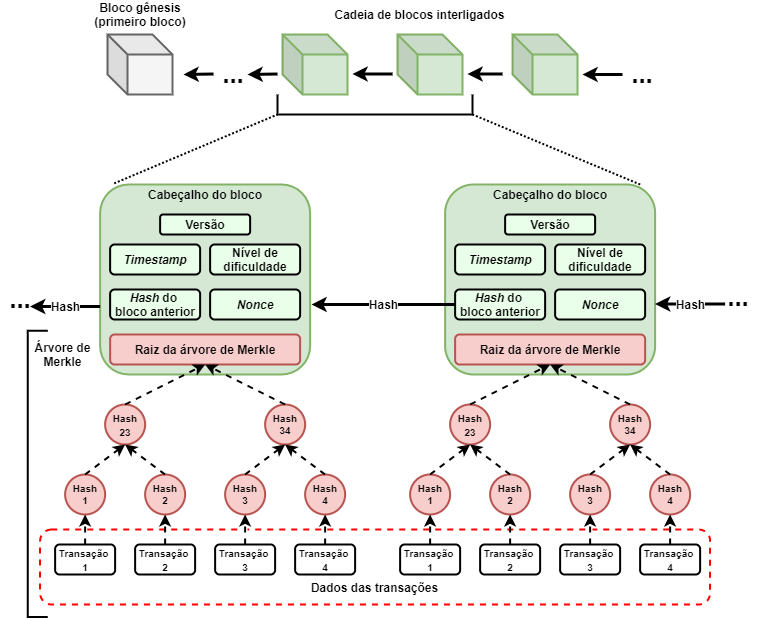
\includegraphics[scale=0.6]{figuras/block_estrutura_cabeçalho.png}
 \fdireta{erikson2020survey-health, overview-dinh-2018}
\end{figure}

Para cada bloco é criado um cabeçalho, que passa a integrar o bloco. As informações presentes no cabeçalho podem variar de acordo com a rede blockchain. Na rede Bitcoin~\cite{overview-bitcoin2008nakamoto}, um cabeçalho é formado por cinco elementos:
\begin{itemize}
    \item \textbf{Versão:} Número da versão do protocolo de regras de validação a ser seguido; 
    \item \textbf{\textit{Hash} do bloco anterior:} Isto é, o código \textit{hash} obtido a partir dos dados do cabeçalho do último bloco presente na blockchain no momento da construção do próximo bloco;
    \item \textbf{Raiz da árvore de Merkle:} Em um bloco, apenas a raiz da árvore de Merkle é armazenada. Desta forma, qualquer tentativa de adulterar ou adicionar indevidamente uma transação na árvore referenciada pelo bloco irá invalidar a referência de \textit{hash} da raiz, alterando também o valor do \textit{hash} do bloco;
    \item \textbf{\textit{Timestamp}:} Horário atual referente ao momento em que o bloco está sendo criado. Esta informação é essencial para manter a ordenação dos blocos no histórico de transações mantido por cada nó da rede;
    \item \textbf{Nível de dificuldade:} Número que indica o nível de dificuldade do quebra-cabeça computacional que deve ser resolvido pelos mineradores na disputa pela criação do próximo bloco. Este item influencia diretamente no tempo e esforço computacional necessário para a criação de um bloco;
    \item \textbf{\textit{nonce}:} Quando o \textit{nonce} é acrescendo ao cabeçalho do bloco, o código \textit{hash} obtido a partir do cabeçalho deve ser iniciado por uma quantidade predefinida de zeros, que é indicada pelo nível de dificuldade. 
\end{itemize}

%%%%%%%%%%% Inserir figura do exemplo do nonce em um bloco

Ao se criar um bloco, o minerador forma primeiro um bloco preliminar contendo os dados dos itens 1 ao 5. Para se obter o \textit{nonce} é necessário realizar uma quantidade massiva de tentativas com o intuito de encontrar a sequência de caracteres e dígitos que satisfaça o nível de dificuldade predefinido. Essa tarefa é conhecidas como mineração, e gera uma disputa entre os nós da rede pela criação do próximo bloco. Nessa disputa, aqueles que possuem computadores mais robustos e com maior capacidade de processamento têm maiores chances de ganhar. A descoberta do \textit{nonce} também é referida neste trabalho como um quebra-cabeça computacional ou quebra-cabeça de \textit{hash}. 

O \textit{nonce} é um item necessário em blockchains nas quais, assim como na \textit{Bitcoin}, utilizam um algoritmo de consenso com regras para criação e validação de blocos conhecido como \textit{proof-of-work}~\cite{overview-bitcoin2008nakamoto}.

Assim que o \textit{nonce} é adicionado ao bloco, este é então transmitido pela rede para que todos os nós possam acessá-lo e participar do processo de validação do bloco. Caso o bloco seja aceito no processo de validação, então cada nó adiciona o bloco válido à própria cópia da estrutura de dados blockchain e o minerador é recompensado pelo gasto que teve~\cite{overview-bitcoin2008nakamoto}.

Como o \textit{hash} gerado nas ramificações da árvore de Merkle depende diretamente do conteúdo das transações, qualquer alteração em uma transação invalida as referências de \textit{hash} dos nós da ramificação da qual a transação pertence, inclusive o nó raiz. Com uma modificação no valor de \textit{hash} da árvore de Merkle, o valor de \textit{hash} do bloco também é alterado. Modificar o valor de \textit{hash} do bloco invalida a referência de \textit{hash} que aponta para o cabeçalho do bloco modificado, invalidando, assim, toda a estrutura de dados.

Desta forma, tentar fraudar dados de transação manipulados envolve uma série de operações custosas. Primeiro deve-se reescrever a árvore de Merkle à qual a transação manipulada pertence. Após isso, é necessário reescrever o cabeçalho do bloco a qual a raiz da árvore de Merkle reescrita pertence, o que requer a solução do quebra-cabeça de \textit{hash} para obtenção de um novo \textit{nonce}. Consequentemente, todos os cabeçalhos até o final da estrutura de dados da blockchain precisam ser reescritos, o que inclui encontrar o \textit{nonce} de cada um. Este processo é propositalmente complexo e se faz necessário para manter os dados consistentes e íntegros. Isso atribui à tecnologia blockchain a propriedade de imutabilidade.

%Elaborar a figura da construção do bloco baseado na imagem de \cite{consenso-Bouraga2021}

%-------------------------------------------------------------------%
\subsection{Tipos de redes blockchain} \label{tex:fund:blockchain:tipo}

%Utilizar a tabela disponível em \cite{overview-ahmed-2019} para comparação entre os tipos de rede

O funcionamento de uma blockchain varia de acordo com a forma como se lida com questões como imutabilidade, permissões, velocidade de processamento de transações  e gerenciamento de participantes no processo de validação. Por isso, existem diferentes variações em blockchains de acordo com as necessidades das aplicações. Baseada nas características descritas por~\citeonline{overview-ahmed-2019} e~\citeonline{overview-consenso2017sankar}, esses tipos de blockchains podem ser classificados com segue:

\begin{itemize}
    \item \textbf{Blockchain pública:} A participação no processo de criação e validação de blocos, assim como o acesso ao histórico de transações, é aberto à todos os nós da rede. Todos os nós são livres para se juntar ou deixar a rede como desejarem. Os exemplos mais conhecidos de blockchain pública são a Bitcoin e a Ethereum, em que os mineradores validam as transações e recebem criptomoedas como recompensa pelo esforço em resolver o quebra-cabeça de \textit{hash};
    \item \textbf{Blockchain privada:} Não é publicamente acessível e possui uma estrutura centralizada. Regras para restrição de acesso e criação de blocos são estabelecidas, controladas e fiscalizadas por uma entidade central. Blockchains privadas são projetadas especialmente para empresas e companhias, como, por exemplo, a blockchain da Ripple~\cite{overview-schwartz2014ripple}. 
    \item \textbf{Blockchain de consórcio:} Nem todos os nós participantes possuem os mesmo direitos de validação de transações e participação no processo de consenso. Apenas o conjunto de nós servidores previamente selecionados podem controlar uma blockchain de consórcio e validar blocos, como acontece nas blockchains Hyperledger Fabric~\cite{overview-hyperledger2018androulaki} e Corda~\cite{brown2016corda}. 
\end{itemize}

Devido à sua natureza aberta para participação, uma blockchain pública é definida também como uma blockchain não permissiva. Já as blockchains privadas e de consórcio concedem direitos de acesso aos dados e validação de transações à nós específicos, e são, portanto, classificadas como blockchains permissivas. Há também casos como o da Ethereum, que, mesmo sendo uma blockchain utilizada como pública, também é possível configurar ambientes privados com controle de acesso. Maiores detalhes sobre a rede Ethereum são tratados na Seção~\ref{tex:fund:ethereum}.

%---------------------------------------------------------------%
\subsection{Processo de validação na Blockchain} \label{tex:fund:blockchain:consenso}

Um fator fundamental no êxito da Blockchain foi sua capacidade de garantir integridade e confiança em um ambiente de sistemas ponto a ponto puramente distribuídos, onde há um número ilimitado de nós conectados sem nenhum nível de confiança pré-estabelecidos entre estes. Em uma rede de blocos com informações que podem ser produzidas por qualquer nó conectado, há o risco iminente de inserção de informações falsas e maliciosas. Para garantir a confiança de que os blocos na blockchain são legítimos, é necessário verificar a validade de um novo bloco antes deste ser inserido na rede. 

Por meio de um protocolo previamente estabelecido, os nós são responsáveis por chegar a um consenso para validar cada inserção, seguindo a ordem na qual as transações ocorrem. Para incentivar os nós a manterem a integridade das transações, são definidos mecanismos de incentivo, assim como formas de punição para os nós que tentam inserir ou validar transações maliciosas. Em uma blockchain, as regras que regem esse protocolo são definidas por um algoritmo de consenso.

Neste trabalho, o termo ``protocolo de consenso'' é usado para se referir de forma generalizada ao processo de tomada de decisão coletiva entre os nós para validação de novos blocos, um procedimento pertinente em qualquer rede blockchain. Contudo, em cada rede blockchain, esse protocolo pode ser composto por regras distintas. Cada conjunto específico de regras para estabelecimento de um protocolo de consenso é referido neste trabalho como um algoritmo de consenso, que pode apresentar diversas variações.

Um algoritmo de consenso é elaborado com o objetivo de garantir que todos os nós da rede concordem com o histórico da transações que compõem os blocos da rede, que será comum à todos, formando assim a rede blockchain~\cite{consenso-xiao-2020}. Desta forma, os nós são estimulados a participar do processo de validação. Além de proporcionar um ambiente participativo para criação e validação dos blocos, os algoritmos de consenso propõe formas de recompensar os nós honestos, isto é, aqueles que trabalham para manter a integridade da rede e não agem de forma maliciosa. 

Para atingir seu objetivo, um algoritmo de consenso deve ser projetado baseado em determinados requerimentos que visam garantir a integridade em uma rede blockchain. No trabalho de \citeonline{consenso-xiao-2020} são definidos 4 requerimentos:

\begin{itemize}
    \item \textbf{Terminação}: Para cada nó honesto, uma nova transação pode ser descartada ou aceita na blockchain, juntamente do conteúdo de um bloco;
    \item \textbf{Concordância}: Cada nova transação e seu respectivo bloco pode ser aceito ou descartado por todos os nós honestos. Cada nó honesto deve atribuir ao bloco aceito o mesmo número de sequência. Este requerimento controla a disposição na ordem correta dos blocos e transações;
    \item \textbf{Validade}: Se cada nó recebe o mesmo bloco válido, então este bloco é aceito e inserido na blockchain;
    \item \textbf{Integridade}: Para cada nó honesto, todas as transações aceitas devem ser consistentes entre si. Cada bloco aceito deve ser gerado e inserido na blockchain em ordem cronológica, ligado ao último bloco da rede por meio de sua referência de \textit{hash}.
\end{itemize} 

Os requerimentos de terminação e validade representam a propriedade de vivacidade da rede, pois fazem com que todos os nós honestos participem do processo de recebimento e integração de novos blocos, agregando valor ao processo de consenso. A concordância garante que todos os nós tenham acesso à mesma estrutura de dados blockchain. Assim, a sequência de blocos e transações deve ser a mesma para todos os participantes. Por meio do requerimento de integridade se estabelece a exatidão da origem de transações e blocos, visando evitar ataques como o gasto duplo, o que reforça a consistência e segurança da rede~\cite{consenso-xiao-2020, consenso-Bouraga2021}.

Cada protocolo de consenso pode dispor de diferentes mecanismos para cumprir com os requerimentos citados, e a forma de implementar cada um desses varia de acordo com a rede blockchain. Contudo, cinco componentes básicos podem ser destacados, como feito por~\citeonline{consenso-xiao-2020}: 

\begin{itemize}
    \item \textbf{Proposta do bloco}: Geração dos blocos e incorporação das provas da execução deste processo;
    \item \textbf{Propagação da informação}: Disseminação dos blocos a transações pela rede;
    \item \textbf{Validação do bloco}: Checagem dos blocos para produção de provas da geração dos blocos e da validade das transações;
    \item \textbf{Finalização do bloco}: Atingir um acordo para aceitação dos blocos válidos;
    \item \textbf{Mecanismo de incentivo}: Atribuir recompensas para os nós honestos participantes e geração de criptomoedas.
\end{itemize}

Cada blockchain pode utilizar uma variação de diferentes algoritmos de consenso. Dentre os principais algoritmos de consenso estão o \sigla{PoW}{\textit{Proof-of-Work}}, \sigla{PoS}{\textit{Proof-of-Stake}} e \sigla{PBFT}{\textit{Practical Byzantine Fault Tolerance}}.

\begin{itemize}
    \item \textbf{\textit{Proof-of-Work}}: O algoritmo \textit{Proof-of-Work} tem entre seus principais mecanismos a competição entre os nós participantes do processo de validação (chamados de mineradores) para resolução de um quebra-cabeça criptográfico. O nó que encontrar uma solução primeiro obtém o direito de validar o bloco, que é então criado, dissipado pela rede de nós para que todos os participantes possam verificar sua validade, e, por fim, o nó é adicionado à blockchain. Para estimular a participação honesta dos nós no processo de mineração e compensar os custos financeiros envolvidos neste processo, visto que o esforço computacional exigido tem como consequência um alto consumo de energia, algoritmos de PoW utilizados em blockchains como Bitcoin e Ethereum oferecem uma recompensa ao vencedor. Esta recompensa é feita por meio da obtenção da posse, por parte do minerador, de uma quantidade da moeda virtual utilizada como incentivo na rede, que pode posteriormente ser convertida em valor monetário (i.e., alguma moeda fiduciária)~\cite{overview-bitcoin2008nakamoto, ethereum2014whitepaper, overview-blockchainbasic2018drescher}. O alto esforço computacional e gasto energético despendido pelos mineradores agrega integridade aos blocos, pois não é vantajoso para um nó malicioso ter um alto gasto para resolução do quebra-cabeça criptográfico de um bloco contendo transações fraudadas e correr o risco iminente do bloco ser rejeitado no processo de validação entre os nós da rede. Por outro lado, o gasto computacional elevado para manutenção da integridade da \textit{blokchain} pode restringir as condições de acesso dos usuários ao processo de mineração, além de aumentar o tempo para inclusão das transações, limitando questões práticas de implantação e uso de sistemas, como escalabilidade e performance~\cite{consenso-Bouraga2021};
    \item \textbf{\textit{Proof-of-Stake}}: O algoritmo PoS foi proposto inicialmente por \citeonline{overview-pos-king2012ppcoin} com o intuito de mitigar a dependência do alto consumo de energia e recursos computacionais do PoW~\cite{overview-bitcoin-energy2014}. No PoS, os nós que se candidatam para participar da criação dos blocos, chamados de validadores, investem uma quantia da criptomoeda vigente na blockchain. Esta quantia também é referida como valor de participação, e funciona como uma conta bloqueada com um saldo que representa o comprometimento do validador em manter a integridade da rede. Quanto maior o valor, maior a chance do validador ser selecionado para criar o próximo bloco. Enquanto no PoW a chance do minerador criar um bloco é proporcional ao seu poder computacional, no PoS a chance é proporcional ao valor de participação investido pelo validador~\cite{consenso-xiao-2020, overview-dinh-2018}; 
    \item \textbf{\textit{Practical Byzantine Fault Tolerance}}: Baseado no trabalho de \citeonline{overview-byzantine1999castro}, o PBFT é adotado na blockchain por meio de dois tipos de nós, o cliente e o servidor. O nó cliente envia um bloco aos nós servidores, e se o bloco for validado por um número suficiente de nós, então este é adicionado à blockchain. Este processo de validação das transações do PBFT consiste em cinco etapas: (i) o nó cliente envia o bloco proposto para os servidores; (ii) os servidores transmitem o bloco para outros servidores, que devem avaliar uma série de condições relacionadas à validade do bloco e chegar a um consenso sobre sua aceitação; (iii) Se o bloco for aceito, o segundo grupo de servidores enviam uma mensagem aos outros nós indicando que o bloco está pronto. Assim que esta mensagem é verificada e validada por um número suficiente de nós, estes entram em fase de ``entrega''; (iv) após realizar a confirmação, cada nó transmite uma mensagem para a rede para atestar sua ação; e (v) o nó servidor que enviou o bloco recebe a resposta, seja o bloco validado ou não~\cite{consenso-Bouraga2021,consenso-xiao-2020,overview-ahmed-2019,consenso-zhang2020analysis}. 
\end{itemize} 

Apesar de ser crucial para o sucesso de blockchains como Bitcoin e Ethereum, o algoritmo PoW impõe limitações de escalabilidade, performance e participação na rede. Essas questões motivaram pesquisadores e empresas a desenvolver alternativas para mitigação desses problemas, como os algoritmos PoS e PBFT. 

Em dezembro de 2020 começou a primeira fase de implantação da \textit{Ethereum} 2.0~\footnote{\url{https://github.com/ethereum/eth2.0-specs}}, uma nova rede blockchain que utiliza o algoritmo de consenso PoS. Com isso, pretende-se aumentar a velocidade de validação das transações e integração dos blocos, expandindo a escalabilidade e otimizando a performance das aplicações.

O algoritmo PBFT é utilizado pela \textit{Hyperledger Fabric}~\footnote{\url{https://www.hyperledger.org/use/fabric}}, uma plataforma blockchain privada desenvolvida pela Fundação Linux~\cite{overview-hyperledger2018androulaki}. Assim como o PoS, o PBFT também proporciona economia de energia para validação e integração das transações. Variações do PBFT também são empregadas nas blockchains Stellar~\cite{overview-stellar2015mazieres} e Ripple~\cite{overview-schwartz2014ripple}~\cite{overview-ahmed-2019, consenso-xiao-2020, consenso-zhang2020analysis}.
 
%------- Parágrafo descartado ---------
%Os protocolos de consenso desempenham um papel crucial para o sucesso das tecnologias baseadas em blockchain. A rede Bitcoin, especificada por \citeonline{overview-bitcoin2008nakamoto}, aliou diversos conceitos para descrição do algoritmo de consenso PoW, o que fez do Bitcoin o foi o primeiro caso de sucesso de uma tecnologia capaz de fornecer integridade e segurança em um sistema ponto a ponto puramente distribuído para gerenciamento de posses (i.e., da criptomoeda Bitcoin). Porém, problemas relacionados com o alto gasto em \textit{hardware} e energia para criação dos blocos, e com a espera significativa para integração dos blocos na rede (em torno de 10 minutos na Bitcoin).

\subsection{Escolha do histórico de transações}

O funcionamento da blockchain exige um ritmo de trabalho dos mineradores no qual, em algum momento, estes sempre estarão concentrados em alguma das seguintes tarefas: analisar um novo bloco criado por algum nó da rede; ou se esforçar para criar o próximo bloco que, posteriormente, será analisado pelos demais nós.

A capacidade de transmissão e entrega de novos blocos sofre grande influência da capacidade da entrega de mensagens de rede. Por consequência, vários nós podem terminar de construir um bloco em um pequeno intervalo de tempo. Esses blocos são transmitidos pela rede e coletados pelos nós em momentos distintos. Assim, os nós da rede não terão informações idênticas à sua disposição ao mesmo tempo~\cite{overview-blockchainbasic2018drescher}. 

Quando um nó coleta um sua caixa de entrada mais de um nó com o mesmo valor de referência do \textit{hash} do bloco anterior, então uma ramificação, referida também como um \textit{fork}, é criada, já que esses blocos possuem o mesmo bloco pai. Essas ramificações podem formar uma cadeia com diversos blocos. Dessa forma, a estrutura de dados da blockchain pode ser vista como uma árvore, porém, quando ocorre um \textit{fork}, os nós da rede devem escolher apenas uma ramificação para compor a cadeia de blocos principal. Na Bitcoin é definido que, sempre que ocorrer um \textit{fork}, deve-se escolher a cadeia mais longa, ou, em caso de empate, mantém-se aquela que foi recebida primeiro.~\cite{overview-blockchainbasic2018drescher, sompolinsky2015ghost-original}.

%Assim, a ramificação com mais blocos interligados é escolhida. Como o algoritmo PoW exige uma disputa entre os mineradores que envolve poder computacional para a criação de um bloco, então a ramificação com mais blocos é também aquela com o maior esforço computacional dispendido~\cite{overview-bitcoin2008nakamoto}.  

Em situações de decisão como essa, o protocolo da Bitcoin estabelece que a ramificação escolhida pela maioria dos nós é considerada como parte da cadeia de blocos principal, como ilustrado na Figura~\ref{fig:cadeia_blocos}. Este procedimento é estabelecido pelo protocolo de consenso da blockchain e visa manter a integridade da blockchain por meio do consenso alcançado entre os nós participantes. Porém, deve-se considerar a premissa de que sempre haverá mais de 50\% de participantes dispostos a agir de forma honesta~\cite{overview-bitcoin2008nakamoto}. 

\begin{figure}[htb]
 \caption{Cadeia de blocos de uma blockchain}
 \label{fig:cadeia_blocos}
 \centering
 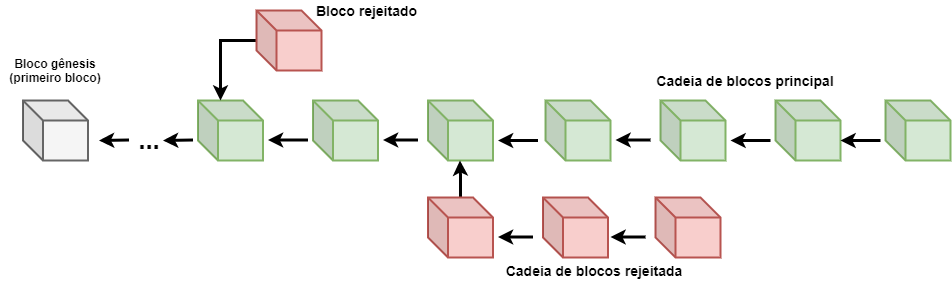
\includegraphics[scale=0.4]{figuras/cadeia_de_blocos.png}
 \fdireta{monrat2019survey-blockchain-ieee}
\end{figure}
 
%-------------------------------------------------------------%
\subsection{Criptografia e autorização de transações} \label{tex:fund:blockchain:cripto}

Em uma blockchain pública qualquer nó pode criar transações e submetê-las para validação, enquanto que em uma blockchain privada essa atividade pode ser autorizada à apenas um conjunto de nós. Independente do acesso de leitura e escrita concedido, é essencial que apenas o proprietário legítimo de uma conta possa transferir o direito de propriedade ou de posse associado à sua conta (e.g., uma quantia de criptomoeda) para outra conta. 

Para garantir que somente o proprietário legítimo transfira a posse, é utilizada uma assinatura digital. Para isso, é aplicada a criptografia de curva elíptica~\cite{koblitz1987elliptic-curve}, na qual são utilizadas técnicas de \textit{hash} e criptografia assimétrica por meio do par de chaves que cada nó detém, uma chave pública e outra privada. A chave privada fica disponível apenas para seu proprietário, e é utilizada para criptografar informações, transformando-as em um texto cifrado. Por se tratar de uma criptografia assimétrica, não há como se obter a informação original por meio do texto cifrado resultante. A única forma de descriptografar esse texto e obter novamente a informação original é utilizando a chave pública correspondente, que é única para cada proprietário e representa o identificador de sua conta. A chave pública é compartilhada com todos, assim, qualquer nó pode usá-la para se certificar de que a transação foi autorizada por quem cedeu a posse~\cite{overview-blockchainbasic2018drescher}.

A assinatura é utilizada em duas situações: na assinatura de uma transação; e na verificação de uma transação~\cite{overview-blockchainbasic2018drescher}. Na Figura~\ref{fig:retemente-assinatura-digital} é ilustrado um exemplo em que o proprietário da conta que cede a posse realiza a assinatura da transação por meio de dos passos a seguir:
\begin{enumerate}
    \item Descreve a transação com todas a informações necessárias, exceto a assinatura;
    \item Gera o valor de \textit{hash} dos dados de transação;
    \item Utiliza sua chave privada para gerar o valor de \textit{hash} da transação a partir do valor gerado no passo 2. Esse processo é chamado de encriptação;
    \item Adiciona o texto cifrado criado no item 3 à transação como sua assinatura digital.
\end{enumerate}

\begin{figure}[htb]
 \caption{Processo de assinatura digital de uma transação}
 \label{fig:retemente-assinatura-digital}
 \centering
 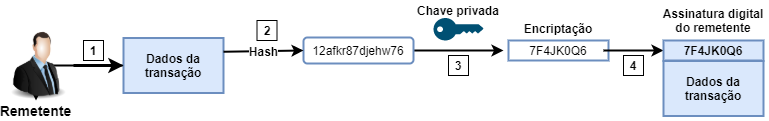
\includegraphics[scale=0.5]{figuras/remetente_assinatura_digital.png}
 \fdireta{overview-ahmed-2019}
\end{figure}

O processo de verificação de uma transação é ilustrado na Figura~\ref{fig:verifica-assinatura-digital}, no qual o nó verificador executa os seguintes passos:
\begin{enumerate}
    \item Cria o valor de \textit{hash} a partir dos dados da transação a ser verificada, com exceção da assinatura;
    \item Utiliza a chave pública da conta que está cedendo a posse para descriptografar a assinatura digital da transação. Esse processo é chamado de decriptação;
    \item Compara o valor do \textit{hash} gerado no passo 1 com o valor obtido no passo 2. Se ambos forem idênticos, então indica que a transação foi autorizada pelo proprietário da chave privada, que corresponde à chave pública que está cedendo a posse (i.e., o identificador da conta). Caso os valores não sejam idênticos, então conclui-se que o proprietário da chave privada não autorizou a transação, que é descartada. 
\end{enumerate}

\begin{figure}[htb]
 \caption{Processo de verificação da assinatura digital de uma transação}
 \label{fig:verifica-assinatura-digital}
 \centering
 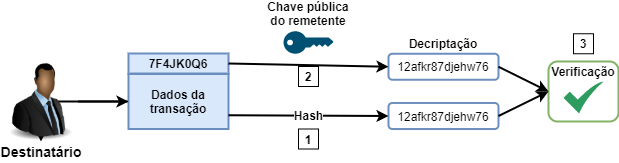
\includegraphics[scale=0.5]{figuras/verifica_assinatura_digital.png}
 \fdireta{overview-ahmed-2019}
\end{figure}

Um valor de \textit{hash} criptográfico é único para cada transação. Analogamente, a associação entre uma chave pública e uma privada também é único. Essa característica faz com que as assinaturas digitais sejam apropriadas para servir como prova de que o proprietário da chave privada usada para criar a assinatura digital realmente concorda com o conteúdo da transação~\cite{overview-blockchainbasic2018drescher}.

%------------------------------------------------------------%
\subsection{Bitcoin como um sistema de transição de estados} \label{tex:fund:blockchain:transition_system}

Do ponto de vista técnico, um livro-razão para gerenciamento de posses de criptomoedas, como o da Bitcoin, pode ser considerado como um sistema de transição de estados. Este estado consiste no status da posse de todos os bitcoins existentes, e uma mudança de estados acontece sempre que uma solicitação de transferência de posse da moeda é aceita, alterando o status de posse das mesmas. No sistema bancário tradicional, seria como transferir uma quantia de dinheiro de uma conta para outra, alterando o estado destas contas, que passam a ter um novo valor de saldo~\cite{ethereum2014whitepaper}.

O estado da Bitcoin é representado pelo conjunto de todas as saídas de transações não gastas, denominadas como \sigla{UTXO}{\textit{unspent transaction outputs}}, que representam todas as moedas já mineiradas. Para cada UTXO é atribuído o endereço de seu proprietário, isto é, a chave pública criptográfica de um nó. Cada transação é composta por ao menos uma entrada e saída. Cada entrada contém uma referência para uma UTXO existente e a assinatura digital criptográfica de quem detém sua posse. Uma saída possui uma nova UTXO a ser adicionada ao novo estado~\cite{ethereum2014whitepaper}. 

% inserir imagem da bitcoin como sistema de transição de estados e mencioná-la no texto

%-----------------------------------------------------------------%
\section{Blockchain Ethereum} \label{tex:fund:ethereum}

A Ethereum~\cite{ethereum2014whitepaper} é uma das mais conhecidas implementações da tecnologia blockchain. Ela é definida como uma plataforma de computação distribuída composta por uma rede de computadores que operam de forma descentralizada, autônoma e democrática~\cite{wood2014ethereum-yellow-paper}. Embora também lide com geração e gerenciamento de posse de sua criptomoeda, o Ether, essa é apenas uma parte do que a plataforma é capaz de prover.

O funcionamento da Ethereum baseia-se na implantação de contratos inteligentes, que são programas de computador que, uma vez implantados, executam automaticamente e obrigatoriamente  de acordo a lógica definida em sua programação. Por meio desses programas é possível estabelecer um acordo entre duas ou mais partes envolvidas, que se comprometem a cumprir com as regras estabelecidas expressas em código~\cite{overview-chen2020blockchain-graph}.

Na Ethereum, as transações são disparadas por meio de mensagens, que podem conter instruções que causam a alteração na estado da blockchain~\cite{wood2014ethereum-yellow-paper}. Isso acontece, por exemplo, quando um nó executa uma função de um contrato inteligente que altera o valor de algum atributo. Essas transações são coletadas pelos nós para formação dos blocos e são estruturadas por meio de uma variação da árvore de Merkle denominada árvore de Patricia Markle, também chamada de \textit{trie}. Esta árvore opera de forma semelhante à arvore de Merkle na garantia de imutabilidade dos dados, pois nela as informações das transações também ficam armazenadas nos nós folhas, assim como os demais nós também são formados pela criptografia do conteúdo de seus nós filhos. Assim, qualquer alteração nos dados de uma transação causa alterações sucessivas nos nós da mesma ramificação, inclusive a raiz.

Contratos inteligentes são geralmente escritos em linguagens de auto nível e Turing-completas, sendo Solidity a linguagem mais utilizada na plataforma Ethereum. A compilação do contrato resulta em um \textit{bytecode}, um código de baixo nível composto por instruções e argumentos. O \textit{bytecode} é então executado nos nós da rede por meio da \sigla{MVE}{Máquina Virtual Ethereum}, uma máquina virtual Turing-completa~\cite{overview-chen2020blockchain-graph, overview-syed2019comparative}.

A Ethereum foi elaborada por~\citeonline{ethereum2014whitepaper} para ser um protocolo alternativo para criação de DApps. Na plataforma \textit{State of The DApps}~\cite{state-dapps-2021} há mais de 3800 DApps contabilizados, sendo que destes, pouco mais de 3 mil utilizam a Ethereum. Nas DApps, geralmente o \textit{front-end} é implementado como uma aplicação \textit{web}, enquanto que o \textit{back-end} é implementado por um ou mais contratos inteligentes~\cite{survey-Hewa2021smart-contract}. Os números envolvendo a plataforma ajudam a dimensionar o tamanho de sua popularidade. Em 2021 o valor de mercado da Ethereum superou 210 bilhões de dólares, sendo a segunda maior plataforma em valor de mercado, atrás apenas da Bitcoin~\cite{coinmarketcap2021}. Também, de acordo com a plataforma Etherscan, há ao menos 2 milhões de contratos inteligentes já executados~\cite{etherscan2020contracts}.
% talvez deva colocar essas informações na introdução

Devido às tecnologias e técnicas que compõe a Ethereum, as aplicações que a utilizam dispõe de uma série de propriedades~\cite{ethereum2014whitepaper, survey-Hewa2021smart-contract}, tais como:
%revisar
\begin{itemize}
    \item Descentralização: Eliminação da necessidade de confiança em uma terceira parte reguladora para execução da lógica do contrato;
    \item Imutabilidade: Uma vez executado, o código não pode ser alterado, assim como as transações resultantes da interação entre os contratos e os nós;
    \item Persistência dos dados: Uma vez inseridas na blockchain, as informações contidas em um bloco estarão sempre disponíveis;
    \item Execução autônoma: A execução de condições programadas e fluxo de eventos a serem realizados são disparados automaticamente conforme o sistema blockchain atinge um determinado estado, garantindo a autonomia da execução. O estado no qual uma ação é disparada é definido na programação do contrato inteligente, em comum acordo com todas as partes envolvidas;
    \item Acurácia: Assim que o contrato inteligente é executado, confia-se que as condições programadas serão cumpridas. A acurácia da execução do que foi programado é garantida por meio da transparência envolvida na execução autônoma, pois assim, vieses humanos e erros que podem acontecer em uma execução centralizada são evitados.
\end{itemize}

A seguir, na Seção~\ref{tex:fund:ethereum:clientes}, são abordados os tipos de contas que operam na plataforma Ethereum. Detalhes sobre as transações e mensagens usadas para a comunicação entre as contas são tratados na Seção~\ref{tex:fund:ethereum:transacao-msgs}. Na Seção~\ref{tex:fund:ethereum:transicao} é apresentada a função de transição de estados da Ethereum. Detalhes sobre a formação dos blocos e seu processo de validação são discutidos nas Seções~\ref{tex:fund:ethereum:blocos} e ~\ref{tex:fund:ethereum:valida}, respectivamente. Alguns exemplos de aplicações baseadas em contratos inteligentes que executam sobre a plataforma Ethereum são discutidos na Seção~\ref{tex:fund:ethereum:aplica}. 

%---------------------------------------------------------%
\subsection{Contas Ethereum} \label{tex:fund:ethereum:clientes}

Diferente do modelo de representação de estados da Bitcoin, que é baseado no estado das moedas mineiradas, na Ethereum, o estado da blockchain é definido pelo estado das contas. O estado de todas as contas define o estado da blockchain, que é atualizado sempre que um novo bloco é adicionado. As contas são necessárias para que haja interação dos usuários com a blockchain por meio das transações~\cite{ethereum-homestead2020documentation}. Uma conta pode ser de dois tipos: \sigla{CPE}{Contas de Propriedade Externa}; e \sigla{CC}{contas de contrato}. 

Uma CPE é usada para armazenar os fundos do usuário em Wei, que é a menor sub-denominação de um Ether, sendo um Ether equivalente a $10^{18}$ Wei. As CPEs são associadas e controladas por uma chave privada, e são necessárias para que um cliente possa participar da rede. As CCs são controladas pelo código de um \textit{bytecode} executável, que é gerado na compilação de um contrato inteligente. Em uma CPE pode-se enviar mensagens para outras CPEs ou para uma CC, basta criar uma mensagem, assinar digitalmente a transação e transmiti-lá para na rede. Sempre que uma CC recebe uma mensagem seu código é ativado. Uma mensagem enviada à uma CC tem o intuito de executar alguma função em seu código. Essa função pode executar alguma operação de leitura ou escrita em seu armazenamento interno (i.e., suas variáveis), ou até mesmo criar e executar outro contrato inteligente. Embora um contrato inteligente possa ser criado por uma CPE ou uma CC, uma CPE não pode ser criada por uma conta~\cite{ethereum2014whitepaper, chen2020survey-ethereum-acm}. 

O estado global da Ethereum é definido pelo estado de todas as contas. Internamente, o estado global é obtido por meio de um mapeamento entre os endereços das contas (identificadores de 20 bytes) e o estado de cada conta~\cite{wood2014ethereum-yellow-paper}. Ambas as contas possuem um estado dinâmico, definido por: 
\begin{itemize}
    \item \textbf{\textit{nonce}}: indica o número de transações iniciadas pelo proprietário da CPE correspondente, ou, no caso de uma CC, o número de contratos criados pela conta;
    \item \textbf{\textit{balance}}: saldo em Wei sob posse da CPE ou da CC;
    \item \textbf{\textit{storageRoot}}: Valor do \textit{hash} da raiz da árvore de Patricia Merkle, a qual armazena o estado das variáveis do contrato associadas ao bytecode correspondente. Este atributo não é aplicável às CPEs;
    \item \textbf{\textit{codeHash}}: Valor do \textit{hash} do código em \textit{bytecode} da CC correspondente. Este atributo não é aplicável às CPEs.
\end{itemize}

As operações requisitadas em uma transação são executadas por meio da MVE, que pode seguramente verificar a identidade do remetente (i.e., uma CPE), pois, assim como na Bitcoin, as transações também são assinadas por meio da técnica de curva elíptica~\cite{ethereum-homestead2020documentation}.

%--------------------------------------------%
\subsection{Transações e mensagens} \label{tex:fund:ethereum:transacao-msgs}

Na Ethereum, uma transação se refere a um pacote de dados criptograficamente assinado que armazena uma mensagem a ser enviada por uma CPE. Essa mensagem estabelece uma interação entre uma CPE e uma CC, ou outra CPE, e especifica alguma instrução a ser executada. Há dois tipos de transações: mensagens externas enviadas por uma CPE; e mensagens internas enviadas por uma CC. Ambas as mensagens podem ser usadas para transferência de Ether, e criação e execução de contratos inteligentes~\cite{wood2014ethereum-yellow-paper}. Os dois tipos de transações possuem os seguintes atributos:
\begin{itemize}
    \item \textbf{\textit{nonce}:} Utilizado como um contador, pois indica o número total de transações que já foram iniciadas pelo remetente. Ressalta-se que, este item não possui relação ou função semelhante ao \textit{nonce} utilizado nos cabeçalhos dos blocos da blockchain que implementam o algoritmo de consenso \textit{proof-of-work}, abordado na Seção~\ref{tex:fund:blockchain:consenso};
    \item \textbf{\textit{gasPrice}:} Um valor em Wei a ser pago para cada unidade de \textit{gas} utilizada na execução da respectiva transação;
    \item \textbf{\textit{gasLimit}:} O valor máximo em \textit{gas} que o remetente está disposto a pagar como taxa para o minerador que vencer a disputa pela criação do bloco no qual essa transação está inclusa;
    \item \textbf{Destinatário (\textit{to}):} O endereço do destinatário da mensagem, que pode ser uma CPE ou uma CC;
    \item \textbf{\textit{value}:} Valor em Wei a ser transferido ao destinatário da mensagem. Em caso de criação de contrato, indica o valor a ser depositado na nova contra criada;
    \item \textbf{\textit{(v, r, s)}:} Os dados indicam a assinatura do remetente, feita por meio do Algoritmo de Assinatura Digital de Curva Elíptica~\cite{johnson2001elliptic-ethereum}.
\end{itemize}

Uma transação para criação de um contrato inteligente também possui o seguinte item:
\begin{itemize}
    \item \textbf{\textit{init}:} Especifica, por meio de um vetor de \textit{bytes}, o \textit{bytecode} para o procedimento de inicialização da conta. 
\end{itemize}

O \textit{init} é um fragmento do \textit{bytecode} que é executado apenas na criação da contrato, e então é descartado. Quando executado, retorna o corpo do código da conta, que é um segundo fragmento de código que é executado sempre que a conta recebe uma mensagem, seja por meio de uma transação ou devido a uma execução interna do código~\cite{wood2014ethereum-yellow-paper}. 

Já transações com mensagens para transferência de Ether e execução de contratos possuem o seguinte atributo~\cite{wood2014ethereum-yellow-paper}:
\begin{itemize}
    \item \textbf{\textit{data}:} Um vetor de \textit{bytes} com dados de entrada da mensagem. Esses dados podem ser parâmetros de uma função, por exemplo.
\end{itemize}

A execução de uma transação pode resultar em um certo custo computacional. Na Ethereum esse custo é calculado em \textit{gas}, e assim, cada tipo de operação possui um determinado custo para ser executada, que varia de acordo com a quantidade de passos computacionais envolvidos, além de um custo fixo de 5 \textit{gas} para cada \textit{byte} dos dados da transação~\cite{wood2014ethereum-yellow-paper}. A utilização do \textit{gas} como métrica é benéfica na medida que desvincula o custo computacional envolvido na execução das operações do custo do Wei, que possui valor monetário e está sujeito a variações de mercado. Assim, um cliente pode levar este último fator em consideração no momento de decidir o quanto está disposto a pagar em Wei por unidade \textit{gas} utilizada (\textit{gasPrice}).

O atributo \textit{gasLimit} é essencial para evitar que estruturas de repetição consumam \textit{gas} indefinidamente ou zerem o saldo do remetente, evitando assim maiores perdas. Contratos inteligentes são executas em uma MVE, definida por ~\citeonline{overview-chen2020blockchain-graph} como uma máquina quase Turing-completa. O termo ``quase'' refere-se ao fato de que a execução é limitada à quantidade de \textit{gas} oferecida nas transações~\cite{overview-chen2020blockchain-graph}.

%--------------------------------------------------%
\subsection{Função de transição de estados} \label{tex:fund:ethereum:transicao}

Na Ethereum, o estado global da blockchain é definido pelo estado das contas, seja uma CPE ou uma CC. Quando uma transação é executada, algum atributo de uma conta é alterado. Esse atributo pode ser o saldo em Ether após a realização de uma transferência, ou também o valor de uma variável de um contrato inteligente, por exemplo. Desta forma, ao executar uma transação ($TX$), ocorre uma transição de um estado ($S$) para outro estado ($S'$)~\cite{ethereum2014whitepaper}.

Ao se executar de uma função ($F$) de transição de estado $F(S, TX) \rightarrow S'$, a seguinte sequência de passos deve ser realizada:
\begin{enumerate}
    \item Checar se a transação contém todos os atributos necessários;
    \item Checar se a assinatura digital é válida; 
    \item Checar se o \textit{nonce} da transação e da conta do remetente são iguais. Em caso negativo para algum dos 3 primeiros passos, uma mensagem de erro é retornada;
    \item Calcular a taxa de execução da transação ($gasLimit * gasPrice$); 
    \item Identificar o remetente por meio da assinatura digital;
    \item Subtrair a taxa do saldo da conta e incrementar o \textit{nonce} do remetente. Caso o saldo não seja suficiente, uma mensagem de erro é retornada;
    \item Definir $gas = startGas$, e retirar a quantidade de \textit{gas} a ser paga pelos \textit{bytes} da transação;
    \item Transferir a quantidade de Ether especificada na transação da conta do remetente para a conta do destinatário. Se a conta do destinatário não existir, então esta deve ser criada. Se a conta do destinatário for uma CC, executar o código do contrato até que a execução esteja completa, ou até atingir o limite definido em \textit{gasLimit};
    \item Se a transferência falhar por conta de saldo insuficiente do remetente ou por \textit{gasLimit} atingido, todos os estados alterados são revertidos, exceto o pagamento das taxas dos mineradores, que devem receber o valor em suas contas;
    \item Se a transferência for bem executada, então o remetente recebe de volta a quantia de \textit{gas} restante, e o minerador recebe a taxas referente ao \textit{gas} consumido.
\end{enumerate}

% se der tempo, inserir uma imagem com um exemplo de transição de estados quando uma transação é executada

%-----------------------------------------------------%
\subsection{Blocos} \label{tex:fund:ethereum:blocos}

Na Ethereum, os mineradores agrupam as transações em blocos. O cabeçalho de um bloco da Ethereum contém as seguintes informações:
\begin{itemize}
    \item \textbf{\textit{parentHash}:} Valor do \textit{hash} do cabeçalho do último bloco pai, isto é, o antecessor do bloco atual;
    \item \textbf{\textit{ommersHash}:} Valor do \textit{hash} dos cabeçalhos dos blocos cujo antecessor são iguais ao antecessor do bloco atual. Essas blocos são chamados de \textit{ommers}; 
    \item \textbf{\textit{beneficiary}:} O endereço do minerador deste bloco. Assim, o minerador é identificado e recebe as taxas de mineração coletadas;
    \item \textbf{\textit{stateRoot}:} Valor do \textit{hash} da raiz da \textit{trie} que contém os estados das transações, após todas serem executadas e finalizadas; 
    \item \textbf{\textit{transactionsRoot}:} Valor do \textit{hash} da raiz da \textit{trie} que contém as transações que compõem o bloco; 
    \item \textbf{\textit{receiptsRoot}:} Valor do \textit{hash} da raiz da \textit{trie} que contém os recibos com as informações da execução de todas as transações listadas neste bloco;
    \item \textbf{\textit{logsBloom}:} Contém um \textit{Bloom filter}, uma estrutura de dados probabilística usada para testar se um dado elemento é membro de um conjunto. Neste caso, a estrutura é usada para armazenar informações dos \textit{logs} de entrada dos destinatários de cada transação listada no bloco;
    \item \textbf{\textit{difficult}:} Representa o nível de dificuldade para mineração do bloco. Este item é ajustado dinamicamente à cada novo bloco minerado com o objetivo de manter uma média de 15 segundos para o tempo de validação de cada bloco;
    \item \textbf{\textit{number}:} Número de blocos antecessores a este na estrutura de dados blockchain, considerando o primeiro bloco, chamado de bloco gênesis, como bloco zero;
    \item \textbf{\textit{gasLimit}:} Limite de gastos de \textit{gas} por bloco;
    \item \textbf{\textit{gasUsed}:} Soma de todo \textit{gas} utilizado pelas transações deste bloco;
    \item \textbf{\textit{timestamp}:} O horário do início deste bloco, definido a partir do padrão \textit{Unix};
    \item \textbf{\textit{extraData}:} Dados extras relacionados a este bloco;
    \item \textbf{\textit{mixHash}:} Valor do \textit{hash} que, quando combinado com o \textit{nonce}, prova que um esforço computacional suficiente foi empregado para a criação deste bloco;
    \item \textbf{\textit{nonce}:} Um valor que, quando combinado com o \textit{mixHash} prova que um esforço computacional suficiente foi empregado para a criação deste bloco. É utilizado junto com o \textit{mixHash} como parte do algoritmo de consenso PoW.
\end{itemize}

Ao se programar um contrato inteligente, pode-se definir e emissão de  \textit{logs}, que são mensagens utilizadas para rastrear quando determinados eventos acontecem durante a execução do código. Esse evento pode ser, por exemplo, uma transferência bem sucedida entre duas contas, ou a criação de um contrato. Uma entrada de \textit{log} contém o endereço da conta responsável pelo disparo da mensagem, tópicos que representam os eventos realizados pela transação, e demais dados associados a esses eventos~\cite{solidity-v7.4-documentation}. O \textit{logsBloom} é o componente do bloco em que esses \textit{logs} são armazenados.

A estrutura do bloco é ilustrada na Figura~\ref{fig:eth-block-header}. Observa-se que são utilizadas três estruturas em árvore para armazenamento das informações resultantes da execução das transações: \textit{stateRoot}; \textit{transactionsRoot}; e \textit{receiptsRoot}. Desta forma, pode-se rastrear em detalhes o processo de execução de cada transação, o que agrega à Ethereum transparência, auditabilidade e persistência dos dados. 

\begin{figure}[htb]
 \caption{Estrutura do cabeçalho de um bloco da Ethereum}
 \label{fig:eth-block-header}
 \centering
 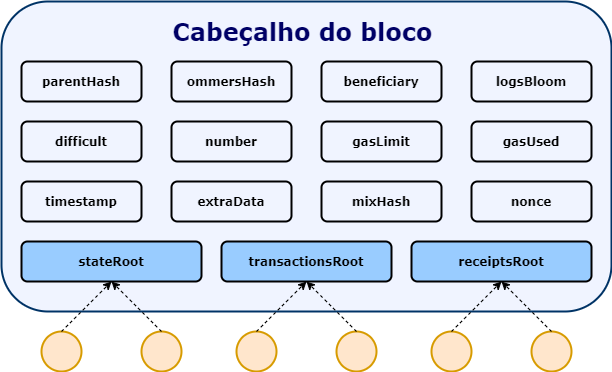
\includegraphics[scale=0.5]{figuras/eth_block_header.png}
 \fdireta{wood2014ethereum-yellow-paper}
\end{figure}

%Trie é a estrutura de dados para armazenar os dados da blockchain Ethereum (como os estados das contas)~\cite{wood2014ethereum-yellow-paper}. Uma árvore trie armazena pares de (chave, valor), facilitando a busca. O caminho da raiz até uma folha corresponde à chave, e os nós folha indicam um valor.

%---------------------------------%
\subsection{Validação} \label{tex:fund:ethereum:valida}

Em uma blockchain, antes de um bloco ser adicionado à cadeia de blocos, este deve passar por um processo de validação por meio de um algoritmo de consenso distribuído. Este processo visa manter a integridade do histórico de transações executadas. Desta forma, cada bloco têm sua integridade verificada pelos nós da rede. Se a maioria dos nós atestarem a integridade do bloco, então este é adicionado na rede principal.

Assim como na Bitcoin, na Ethereum os blocos também podem ser finalizados, transmitidos e recebidos em momentos distintos pelos mineradores, gerando assim um \textit{fork} com versões distintas do histórico de transações. Na Ethereum é utiliza uma variação do protocolo GHOST~\cite{sompolinsky2015ghost-original} para selecionar como parte da rede principal a ramificação com a maior dificuldade de bloco acumulada, enquanto que as demais sub-redes continuam existindo, mas sem fazer parte da rede principal. 

Para cada ramificação, pode-se calcular a dificuldade acumulada, chamada também de ``o caminho mais pesado'', por meio do acesso às informações contidas no cabeçalho do último bloco adicionado. Como o cabeçalho do bloco contém a dificuldade de mineração do bloco, representada pelo campo \textit{difficult}, basta somar recursivamente o valor da dificuldade de mineração de todos os blocos da rede, com o exceção dos bloco gênesis~\cite{wood2014ethereum-yellow-paper}.

Na plataforma Etherscan~\cite{etherscan2020contracts} são coletadas informações sobre todos os blocos e transações incluídos na blockchain Ethereum. Na Figura~\ref{fig:eth-block-difficulty} pode-se observar que, entre outras informações do bloco, há o campo \textit{Total Difficulty}, sublinhado em vermelho, que mostra o valor da dificuldade acumulada na blockchain até o respectivo bloco.

\begin{figure}[htb]
 \caption{Dificuldade acumulada de um bloco na Ethereum}
 \label{fig:eth-block-difficulty}
 \centering
 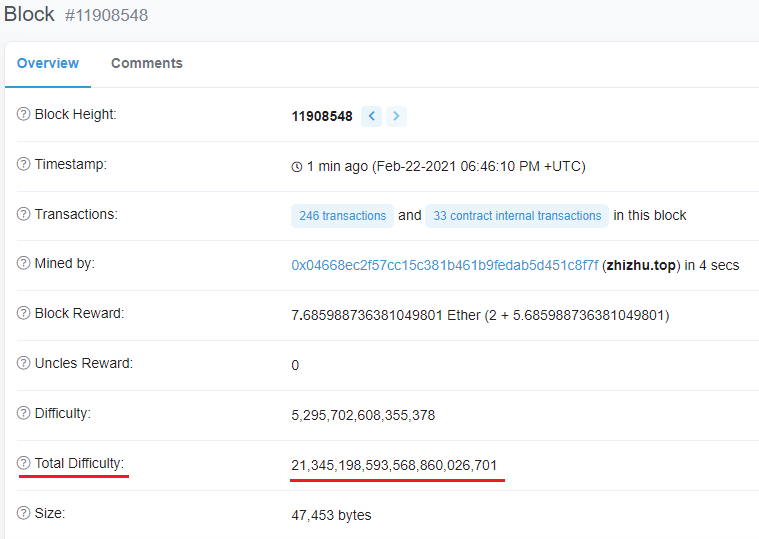
\includegraphics[scale=0.6]{figuras/block-eth-difficulty.png}
 \fdireta{etherscan2020contracts}
\end{figure}

%Em \cite{wang2019survey-consenso} tem uma explicação bem detalhada sobre o funcionamento do quebra-cabeça de hash da ethereum

%-------------------------------------------------------%
%\subsection{Máquina Virtual Ethereum}


%-------------------------------------------------------%
\subsection{Aplicações} \label{tex:fund:ethereum:aplica}

A tecnologia blockchain foi proposta inicialmente com o intuito de apoiar o desenvolvimento de criptomoedas como a Bitcoin. O êxito da Bitcoin chamou atenção tanto da academia quanto da indústria, e, posteriormente, outros tipos de criptomoedas e tecnologias baseadas na blockchain foram desenvolvidas. Como exposto por~\cite{swan2015blockchain-book} e~\cite{maesa2020blockchain3.0}, esses avanços são classificados como \textit{Blockchain 1.0}, \textit{2.0} e \textit{3.0}. blockchains aplicados ao para gerenciamento de posse de criptomoedas integram um conjunto de aplicações classificado como \textit{Blockchain 1.0}. 

Com a introdução dos contratos inteligentes, impulsionados principalmente pela blockchain Ethereum, possibilitou-se a implementação dos DApps. Desta forma, viabilizou-se o uso de sistemas descentralizados projetados para automatizar aplicações financeiras baseadas em criptomoedas, como OADs e sistemas de \textit{tokens}. Tais aplicações são baseadas na junção entre contratos inteligentes e criptomoedas, e são definidas como \textit{Blockchain 2.0}~\cite{maesa2020blockchain3.0}.

\textit{Blockchain 3.0} é o estágio evolucionário no qual a tecnologia não se limita apenas à aplicações financeiras, mas também à áreas como cuidados médicos, ciências, inteligência artificial, internet das coisas, governança descentralizada, entre outras~\cite{maesa2020blockchain3.0}. 

A seguir, nas Seções~\ref{tex:fund:ethereum:app:tokens} e ~\ref{tex:fund:ethereum:app:oad} são abordadas algumas áreas de aplicação da tecnologia blockchain, como sistemas de tokens e OADs, que integram a \textit{Blockchain 2.0}. Na Seção~\ref{tex:fund:ethereum:app:health} é discutido sobre o uso da blockchain para solucionar alguns problemas encontrados na área de cuidados médicos e serviços de saúde. Ao longo das Seções~\ref{tex:fund:ethereum:app:tokens}, ~\ref{tex:fund:ethereum:app:oad} e ~\ref{tex:fund:ethereum:app:health} são citados alguns exemplos de sistemas relacionados com as aplicações tratadas. Como a plataforma Ethereum faz parte do foco e do escopo deste trabalho, são citados apenas exemplos de aplicações desenvolvidas sobre a Ethereum, apesar de existirem outras blockchains que executam aplicações semelhantes.

\subsubsection{Sistemas de tokens} \label{tex:fund:ethereum:app:tokens}

Um token é um ativo digital e programável gerenciado por um contrato inteligente para ser utilizado em um DApp ou algum projeto específico. Tokens são similares às criptomoedas, porém, enquanto criptomoedas como bitcoin e ether possuem uma blockchain própria para sua mineração e gerenciamento de posse, os tokens são criados sobre a estrutura de uma blockchain já existente~\cite{angelo2020tokens}.

Tokens são usados para representar o direito sobre algo, de forma que esse direito é representado como um artefato digital, um processo conhecido como tokenização. O gerenciamento de posse do token usufrui de benefícios inerentes à estrutura de uma blockchain, como imutabilidade, persistência dos dados, descentralização, anonimato e auditabilidade~\cite{angelo2020tokens, monrat2019survey-blockchain-ieee}. 

Quando um artefato é tokenizado, é possível fracionar seu valor para quem se interessa em obter a posse, assim como já acontece com as criptomoedas tradicionais. Desta forma, facilita-se a entrada de investidores, resultando em um aumento de liquidez dos ativos tokenizados. Além disso, O fato de um token ser programável proporciona o gerenciamento autônomo e a concordância dos direitos dos investidores.~\cite{angelo2020tokens}.

Um exemplo de aplicação de tokens são as \textit{stable coins}, moedas digitais cujo valor é lastreado de acordo com alguma moeda fiduciária ou fundos de investimentos já existentes. Projetos como o Tether~\footnote{Tether: Digital money for a digital age. \url{https://tether.to/}} e USD Coin~\footnote{USDC: the world's leading digital dollar stablecoin. ~\url{https://www.circle.com/en/usdc}} operam com as criptomoedas USDT e USDC, que são lastreadas pela cotação do dólar. Já o Pax Gold~\cite{paxgold-whitepaper}, opera por meio do  PAXG, uma versão tokenizada do ouro físico licenciado e certificado pelas agências \textit{London Bullion Market
Association} e   \textit{London Good Delivery}. Desta forma, é possível comprar frações de onças de ouro, equivalente a aproximadamente 31 gramas de ouro, sem a necessidade de adquirir cofres ou contratar serviços de armazenamento disponíveis em bancos~\cite{paxgold-whitepaper}. 

Entre outros exemplos, vale citar também tokens como o WiBX~\footnote{WiBX: Crypto jumping coin. ~\url{https://www.wibx.io/}}, oferecido como recompensa em sistemas de compartilhamento de produtos, o Aave~\cite{aave-site}, uma criptomoeda utilizada em um sistemas de finanças descentralizadas, e o MCO2~\cite{mco2-moss-whitepaper}, token da companhia ambiental MOSS, usado para obtenção de créditos de carbono. 

A facilidade para programação e o estabelecimento de padrões para criação de tokens, como o padrão ERC-20~\footnote{ERC-20 Token standard. ~\url{https://ethereum.org/en/developers/docs/standards/tokens/erc-20/}}, foram fundamentais para o estabelecimento deste tipo de ativo, o qual abrange diversas aplicações. Na plataforma Etherscan~\footnote{Etherscan. Token Traker. \url{https://etherscan.io/tokens}} pode-se consultar uma lista de tokens, na qual, no momento da escrita deste trabalho, foram encontrados 362,745 tokens, considerando apenas aqueles escritos no padrão ERC-20.

\subsubsection{Organizações Autônomas Descentralizadas} \label{tex:fund:ethereum:app:oad}

Uma OAD é uma organização desenvolvida por meio da tecnologia blockchain que pode ser gerida de forma autônoma, sem a necessidade de confiar em uma autoridade central ou estruturas hierárquicas~\cite{wang2019DAO-survey}. Em uma OAD, todas as regras operacionais e de gerenciamento são programadas em um contrato inteligente e gravadas em uma blockchain. Assim, protocolos de consenso e tokens são utilizados como incentivo para estimular a autonomia operacional, governamental e evolucionária das organizações. Por meio da implantação de uma OAD, espera-se abolir modelos de gerenciamento tradicionais baseados em hierarquia, além de reduzir os custos das organizações com comunicação, gerenciamento e colaboração~\cite{wang2019DAO-survey}.

Em 2016, foi lançado o primeiro OAD, chamado de \textit{The DAO} (sigla para \textit{Decentralized Autonomous Organization}), o maior projeto de \textit{crowdfunding} da época, que em pouco tempo arrecadou cerca de 150 milhões de dólares. Por meio do \textit{The DAO}, propostas de investimento eram submetidas e os participantes compravam tokens que davam direito de participação na aprovação das propostas, assim como receber parte dos lucros gerados~\cite{wang2019DAO-survey}.

Após o \textit{The DAO} outras OAD surgiram, como a \textit{Aragon}~\footnote{Aragon: Next-level communities run on Aragon. ~\url{https://aragon.org/}} e a \textit{Steemit}~\footnote{Steemit. ~\url{https://steemit.com/}}. A \textit{Aragon} é uma plataforma que oferece aos usuários uma infraestrutura para criação e gerenciamento de vários tipos de OADs. A \textit{Steemit} é uma plataforma de mídias sociais baseada em blockchain que, por meio de um sistema de tokens, usuários são recompensados pela criação e curadoria de conteúdos.  

Por se tratarem de plataformas com grande capacidade de arrecadação financeira, as OADs tornaram-se alvo de ataques~\cite{atzei2017survey-attacks-sok}. Em junho 2016 ocorreu o caso conhecido como \textit{The DAO Attack}, no qual um participante malicioso explorou uma falha no contrato e transferiu cerca de 3,6 milhões de Ether para sua conta, o equivalente a 50 milhões de dólares~\cite{siegel-dao-attack}. Este caso teve grande repercussão e chamou a atenção da academia e da indústria, impulsionando estudos e estratégias para detecção e prevenção de vulnerabilidades em contratos inteligentes~\cite{chen2020survey-ethereum-acm, liu2019survey-ieeeaccess}.

\subsubsection{Cuidados médicos e serviços de saúde} \label{tex:fund:ethereum:app:health}

Com a ampla difusão da informatização de processos em variadas áreas, do acesso à \textit{internet}, aliados à popularização de \textit{smartphones} e computadores pessoais, um dos maiores problemas enfrentados diz respeito à proteção dos dados pessoais dos usuários. Entre esses dados pessoais estão as informações de serviços de saúde. O histórico médico contém dados sensíveis de pacientes, que precisam ser compartilhados com médicos, farmácias, seguradoras, e outras partes interessadas da área da saúde. Ao mesmo tempo, essas dados devem ser protegido contra acessos indevidos e manipulados corretamente pelos profissionais da área, que muitas vezes não têm conhecimento técnico para lidar com os dados de forma segura.  Além da preocupação com a proteção dos dados, também há falta de padronização do formato desses dados, que podem enfrentar incompatibilidade no compartilhamento entre instituições médicas, profissionais da saúde, e outras partes interessadas~\cite{maesa2020blockchain3.0}.

Outro problema na área da saúde diz respeito à falsificação e adulteração da composição de medicamentos. De acordo com a Organização \sigla{OMS}{Organização Mundial da Saúde}, em 2017, 1 em cada 10 medicamentos nos países em desenvolvimento eram falsificados ou de baixa qualidade~\cite{oms2017medicamentos}.

Diante desses problemas, diversas soluções foram propostas utilizando como base a tecnologia blockchain, que possui potencial para transformar a área de cuidados médicos e serviços de saúde~\citeonline{mcghin2019blockchain-survey-health, erikson2020survey-health}. 

A tecnologia blockchain pode oferecer uma infraestrutura adequada para integração de dados de prontuários médicos, e outros benefícios proporcionados pela integridade e imutabilidade dos dados. Uma proposta que utiliza contratos inteligentes e a estrutura da Ethereum é o sistema MedRec~\cite{ekblaw2016case-medrec}, utilizado para gerenciamento de registros de prontuário eletrônicos. O MedRed permite que pacientes consultem suas informações de forma acessível e oferece uma estrutura modular que facilita a interoperabilidade com sistemas já existentes, além de gerenciar questões como autenticação, confidencialidade, contabilidade e compartilhamento de dados~\cite{ekblaw2016case-medrec}.

Outros exemplos de aplicações da blockchain na área da saúde são relatados nos trabalhos de ~\citeonline{mcghin2019blockchain-survey-health} e  ~\citeonline{erikson2020survey-health}.

%%%%%%%
%%%%% mais p frente falar tbm do uso com IA e IoT

%--------------------------------------------%
\subsection{Arquitetura em camadas} \label{tex:fund:ethereum:camadas}

% Em \citeonline{fan2020performance} são descrita 5 camadas, com a EVM em uma camada separada de execução

A blockchain Ethereum foi projetada sobre uma série de conceitos, protocolos e procedimentos, que dependem de recursos computacionais e tecnológicos para funcionar. Esse conjunto de elementos compõem a arquitetura da Ethereum. Em seu trabalho, \citeonline{chen2020survey-ethereum-acm} dividem essa arquitetura em quatro camadas: aplicação; dados; consenso; e rede. 

A arquitetura em camadas conta também com elementos presentes no ambiente, relacionados com recursos tecnológicos e infraestrutura, como exposto na Figura~\ref{fig:eth-arquitetura}. Na camada de aplicação estão as contas, que podem ser CPEs ou CCs, os contratos inteligentes, e a MVE, responsável pela execução do \textit{bytecode} gerado na compilação do contrato. A camada de dados consiste nas informações geradas ao longo da execução dos contratos, como transações e \textit{logs} de eventos, e no armazenamento destas, que são acessadas por meio dos blocos. Os mecanismos para validação dos blocos estão incluídos na camada de consenso, no qual um algoritmo de consenso e uma política de incentivos é utilizada para motivar os mineradores a agirem de forma honesta. A camada de rede é a responsável pela comunicação entre os participantes da rede, possibilitando a descoberta de novos nós e a propagação e verificação das informações, essencial para que cada nó possa manter seu histórico de transações atualizado~\cite{chen2020survey-ethereum-acm}.    

\begin{figure}[htb]
 \caption{Arquitetura da blockchain Ethereum e seu ambiente de execução}
 \label{fig:eth-arquitetura}
 \centering
 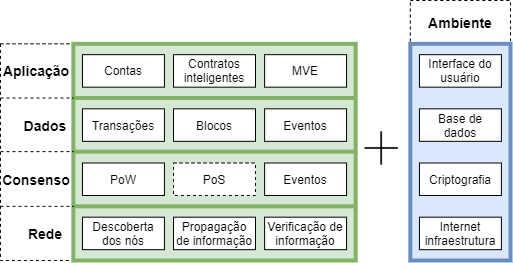
\includegraphics[scale=0.5]{figuras/ethereum_arquitetura.png}
 \fdireta{chen2020survey-ethereum-acm}
\end{figure}

Cada camada depende de componentes do ambiente de execução das aplicações, como uma interface \textit{web} para interação dos usuários com as aplicações, uma base de dados para armazenamento dos dados da blockchain, mecanismos criptográficos para apoiar os protocolos de consenso, e o serviço de \textit{Internet} que dá suporte às tarefas da camada de rede.

Na Figura~\ref{fig:eth-arquitetura}, nota-se que que, na camada de consenso, o retângulo contendo o algoritmo PoS está com o contorno pontilhado. Isto deve-se ao fato da rede Ethereum 2.0, que opera com o algoritmo de consenso PoS, estar em fase inicial de implementação. Futuramente, de acordo com o planejamento do projeto, espera-se que a Ethereum seja englobada pela Ethereum 2.0. 

%%%%%% mais p frente, usar tbm o trabalho ~\cite{zhang2019blockchain-security-acmcs} na fundamentação

\section{Contratos inteligentes} \label{tex:fund:ethereum:smartc}

No trabalho de ~\citeonline{szabo1997smart-contract} foi proposta pela primeira vez a ideia de um contrato inteligente cujas cláusulas são escritas em programas de computador e executadas automaticamente sem a necessidade de confiar em uma terceira parte reguladora. Anos depois, por meio da tecnologia blockchain, os contratos inteligentes puderam ser de fato implementados, impulsionados por plataformas como Ethereum, Hyperledger Fabric, Corda e Stellar~\cite{overview-smartcontracts2020zheng}.

No desenvolvimento de um contrato inteligente, as cláusulas contratuais estabelecidas em comum acordo entre as partes envolvidas são expressas por meio de programas de computador executáveis. Esses programas são normalmente escritos em linguagens de programação de alto nível, como a linguagem Solidity~\cite{solidity-documentation}. Na plataforma Ethereum, independente da linguagem, os contratos inteligentes são sempre convertidos em um \textit{bytecode}, uma linguagem de baixo nível que é executada na MVE.

Na linguagem Solidity, um contrato é similar à um objeto. Cada contrato possui atributos e funções que podem ter seus controles de acesso definidos por modificadores. O controle lógico das condições estabelecidas pelas cláusulas podem ser definidos por meio de estruturas de controle, como \textit{if}, \textit{if-else}, \textit{for}, etc.

Um exemplo de contrato escrito na linguagem Solidity é exposto na Figura~\ref{fig:exemplo-contrato-solidity}. Neste exemplo, a conta que implementa o contrato pode atribuir algum saldo para si ou para outras contas, e esses valores atribuídos podem ser transferidos para outras contas.

\begin{figure}[htb]
 \caption{Contrato escrito na linguagem Solidity para atribuição e transferência de saldo}
 \label{fig:exemplo-contrato-solidity}
 \centering
 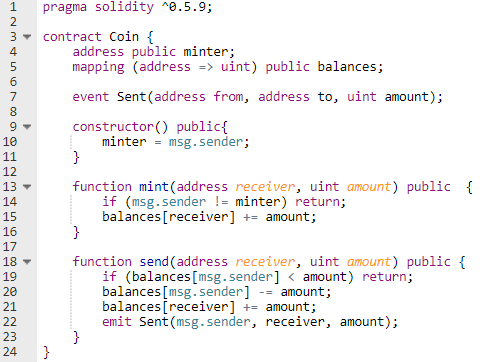
\includegraphics[scale=0.7]{figuras/exemplo_codigo_solidity.png}
 \fdireta{solidity-v5.9-documentation}
\end{figure}

Em seu trabalho, ~\citeonline{overview-smartcontracts2020zheng} descreveram a utilização dos contratos inteligentes como um ciclo de vida que consiste em quatro fases: criação; implantação; execução; e conclusão. Cada fase é descrita como segue:
\begin{enumerate}
    \item \textbf{Criação:} Essa primeira fase se inicia com a negociação entre as partes envolvidas para definição das obrigações, direitos e proibições que devem ser expressas no contrato. Em seguida, desenvolvedores e engenheiros de \textit{software} descrevem esse acordo para alguma linguagem de programação para contratos inteligentes, tal processo para por etapas de projeto, implementação e validação. A criação de contratos inteligentes é um processo interativo que pode envolver a participação de vários profissionais, como investidores, advogados e engenheiros de \textit{software};
    \item \textbf{Implantação:} Consiste em implantar o contrato compilado na blockchain. A implantação é feita por meio de plataformas como a Go Ethereum~\footnote{\textit{Go Ethereum: Official Golang implementation of the Ethereum protocol}. \url{https://github.com/ethereum/go-ethereum}}, que opera sobre a blockchain Ethereum. Uma vez implantado na blockchain o contrato inteligente não pode mais ser modificado, e todas as partes envolvidas podem acessá-lo. Vale ressaltar que, nesta etapa, a partes envolvidas podem ter uma parte de seus bens digitais bloqueados. Esse bem digital pode ser uma quantidade de Ether dada como garantia de uma transferência, por exemplo. Assim, as partes envolvidas podem ser identificadas por meio de suas carteiras digitais; 
    \item \textbf{Execução:} Após a implantação as cláusulas contratuais são monitoradas e avaliadas. Assim, conforme as condições estabelecidas são atingidas, as operações e funções expressas no contrato são automaticamente executadas, o que gera um fluxo de transações que são executadas e validadas pelos mineradores.
    \item \textbf{Conclusão:} Depois que um contrato é executado, o estado das contas das partes envolvidas é atualizado. Logo, as transições e os dados de atualização dos estados são gravados na blockchain, as transferências entre as contas são concretizadas e os bens digitais das partes envolvidas são desbloqueados. Assim, o ciclo de vida de um contrato inteligente é concluído. 
\end{enumerate}

\begin{figure}[htb]
 \caption{Ciclo de vida de um contrato inteligente baseado em 4 fases: criação, implantação, execução e conclusão}
 \label{fig:contrato-ciclo-de-vida}
 \centering
 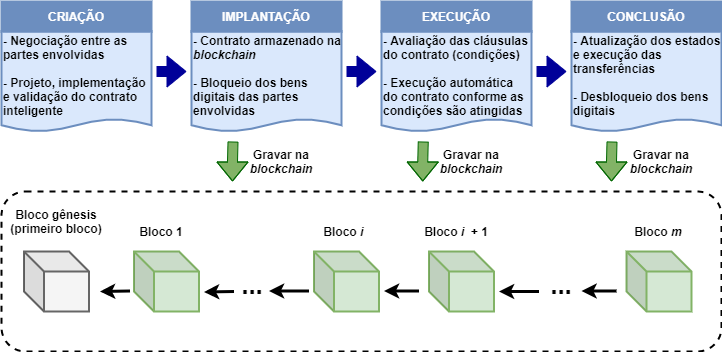
\includegraphics[scale=0.6]{figuras/contrato_ciclo_de_vida.png}
 \fdireta{overview-smartcontracts2020zheng}
\end{figure}

O ciclo de vida dos contratos inteligentes é ilustrado na Figura~\ref{fig:contrato-ciclo-de-vida}. Nota-se que, durante as fases de implantação, execução e conclusão, uma série de transações são geradas, transmitidas, validadas e gravadas na blockchain, proporcionando a rastreabilidade e auditabilidade do contrato~\cite{overview-smartcontracts2020zheng}.

Devido a imutabilidade da blockchain, um contrato implementado não pode mais ser alterado. Esta propriedade agrega integridade à tecnologia blockchain, mas também ressalta a importância da implementação de contratos livres de erros e de acordo com boas práticas, já que vulnerabilidades presentes nos contratos podem torná-los alvos de ataques.

A seguir, na Seção~\ref{tex:fund:ethereum:ataques} são abordadas algumas das vulnerabilidades já encontradas em contratos inteligentes e ataques que ocorreram por meio da exploração dessas vulnerabilidades.  

%-----------------------------------------------------------------------%
\subsection{Vulnerabilidades e ataques} \label{tex:fund:ethereum:ataques}

Aplicações desenvolvidas por meio de contratos inteligentes, como os DApps e as OADs, costumam envolver transferências e gerenciamento de grandes quantidades de bens digitais, e isso tornou-os alvo de uma série de ataques que exploraram vulnerabilidades encontradas no código desses contratos~\cite{atzei2017survey-attacks-sok, liu2019survey-ieeeaccess, chen2020survey-ethereum-acm}.

Há vários fatores que tornam a implementação de contratos inteligentes propícios à erros. Segundo ~\cite{atzei2017survey-attacks-sok}, parte desses erros são ocasionados pelo desalinhamento que há entre a semântica da linguagem Solidity e a intuição dos desenvolvedores. Apesar de alguns elementos em Solidity serem similares aos encontrados em outras linguagens, como o uso de funções, exceções e modificadores de acesso, estes não são implementados da mesma forma.

Desde os primeiros casos notórios de ataques, como o ataque ao The DAO~\cite{siegel-dao-attack}, mencionado na Seção~\ref{tex:fund:ethereum:app:oad}, diversos trabalhos foram desenvolvidos com o intuito de listar e classificar os ataques e as vulnerabilidades explorados em contratos inteligentes, e também relatar os esforços despendidos na mitigação dessas ameaças. 

No trabalho de~\citeonline{chen2020survey-ethereum-acm} são identificadas 40 vulnerabilidades relacionadas com a blockchain Ethereum. Cada vulnerabilidade encontra-se em uma das camadas da arquitetura da Ethereum, a qual é ilustrada na Figura~\ref{fig:eth-arquitetura}. Das vulnerabilidades identificadas, 26 estão na camada de aplicação, que engloba as contas, os contratos inteligentes e a MVE. Destas, 14 estão associadas à programação dos contratos inteligentes. Em outro trabalho, desenvolvido por~\citeonline{atzei2017survey-attacks-sok}, são identificadas 6 vulnerabilidades em contratos escritos na linguagem Solidity, sobre as quais 6 ataques foram realizados. Algumas dessas vulnerabilidades, assim como os respectivos ataques, são descritos no decorrer desta Seção.

\subsubsection*{\textbf{Reentrada}}

Essa vulnerabilidade ocorre quando o contrato de um receptor externo invoca novamente uma função do tipo \textit{callback} de outro contrato antes que este termine de executar essa função. Quando um contrato vulnerável contém uma função \textit{callback}, um contrato externo pode invocá-la sucessivas vezes até esgotar qualquer saldo contido no contrato~\cite{chen2020survey-ethereum-acm, sayeed2020smart-attacks-ieee}. 

A vulnerabilidade da reentrada foi observada primeiramente no \textit{The DAO Attack}, em que um contrato externo transferiu cerca de 3,6 milhões de Ether para sua conta, o equivalente a 50 milhões de dólares~\cite{siegel-dao-attack}. Apesar dos danos terem sido revertidos, isso causou uma divisão entre os mineradores da Ethereum. A maior parte dos mineradores concordaram em reverter os danos por meio de um \textit{hard fork}, um procedimento no qual é feita uma bifurcação na cadeia de blocos, que neste caso, foi referente ao momento anterior ao ataque. Após o \textit{hard fork}, a cadeia de blocos principal da Ethereum continuou a partir do bloco 1920000~\footnote{\textit{Hard Fork Completed}. \url{https://blog.ethereum.org/2016/07/20/hard-fork-completed/}}, enquanto que a outra cadeia foi continuada pelos mineradores que não concordaram com a decisão, e foi denominada como Ethereum Classic~\footnote{Ethereum Classic. \url{https://ethereumclassic.org/}}.  

\subsubsection*{\textbf{Delegatecall Injection}}

Para facilitar o reuso de código, a MVE dispõe do código de operação (do inglês, \textit{opcode}) \texttt{delegatecall}, usado para inserir o \textit{bytecode} de um contrato no \textit{bytecode} de outro contrato, que irá executá-lo por meio de uma chamada. Quando isso ocorre, o contrato que é chamado pode alterar as variáveis de estado do contrato que o invocou. Essa característica torna este último contrato vulnerável à ação de contratos maliciosos que, quando chamados, podem causar alterações para obter benefícios e transferir tokens para sua conta~\cite{chen2020survey-ethereum-acm}.

O primeiro ataque a explorar essa vulnerabilidade ocorreu contra a \textit{Parity Multsignature Wallet}, uma carteira multi-assinatura. Para se autorizar uma transação convencional de Ether, o remetente deve assinar a transação com sua chave privada. Na Ethereum, uma carteira multi-assinatura é um contrato inteligente que requer múltiplas chaves privadas para desbloquear uma carteira e autorizar transferências. Em 2017, uma vulnerabilidade em uma chamada \texttt{delegatecall} foi explorada, e cerca de 31 milhões de dólares em Ether foi subtraído da \textit{Parity Multsignature Wallet}~\cite{chen2020survey-ethereum-acm}.

%Monitoramento em tempo real é pouco explorado \cite{chen2020survey-ethereum-acm} 

% SE DER TEMPO, incluir sessão sobe a execução do bytecode de um contrato na Ethereum Virtual Machine

